\section{Privacy Invasive Services}
\label{sec:characterize-app}

We now use pervasive nature of \platname to detail  the privacy invasiveness of applications and Web-services. 
For our analysis we concentrated on the data sent from the mobile devices with a focus on the {\it what} data is sent,  {\it to whom} is the data sent, and {\it how frequently} is data sent.
%To answer these questions, we rely on the controlled experiments and the \mobWild dataset.

\begin{table*}[t]    
    \centering
    \begin{small}
    \begin{tabular}{|l|l|l|l|l|l|l|l|l|l|}
       \hline
       {\bf Store}&{\bf Platform}&{\bf \# Apps}&{\bf Email}& {\bf Location}& {\bf Name} &{\bf Password}& {\bf Device ID}& {\bf Contacts}& {\bf IMEI}\\
       \hline
       App Store&iPhone&100&13 (13\%) &20 (20\%)&4 (4\%)&0 (0\%)&0 (0\%)&0 (0\%)&1 (1\%)\\
       \hline
       Google Play&Android&100&3 (3\%)&10 (10\%)&2 (2\%)&1 (1\%)&21 (21\%)&0 (0\%)&13 (13\%)\\
       \hline
       Third Party&Android&908&1 (0.1\%)&32 (3.5\%)&2 (0.2\%)&0 (0\%)&95 (10.4\%)&4 (0.4\%)&48 (5.3\%)\\
       \hline
    \end{tabular}
    \end{small}
    \caption{Summary of personally identifiable information leaked in plaintext (HTTP) by Android and iPhone applications. \emph{The popular iOS applications tend to leak the location information in the clear while Android applications leak the IMEI number and Android ID in the clear.}}
    \label{tab:pii}
\end{table*}

\subsection{Personally Identifiable Information Leaks}

For our experiments we created fake user accounts with fake contact information and fake Twitter and Facebook accounts.  
Our objective for was to detect if any personally identifiable information -- email address, phone number, IMEI number -- stored on the device is leaked across the network over HTTP or HTTPS.
While we acknowledge that some of this information may be relevant for the application, we strongly believe that this information should never travel across the network in plaintext (HTTP), which we see violated in several cases.

In \fref{tab:pii}, we present the different personally identifiable information (PII) leaked for both Android and iPhone apps.  
We observe that the IMEI, a unique identifier tied to a phone, is the one of the most commonly leaked PII for Android applications.
Although IMEI is not private, it can be used to track and correlate a user's behavior across the Web-services.
Similarly, we observe that Android application tend to leak the Android ID, a unique identifier tied to an Android device.
In \fref{tab:pii}, we also observe that other information like contacts, email, and passwords were leaked in the clear.
The email address, the address used to sign up for the services, was leaked in the clear by 13 iOS and 3 Android applications from our set of 100 popular applications.


\begin{table}
    \centering
    \begin{small}
    \begin{tabular}{|l|c|c||c|}
       \hline
       {\bf Host}&{\bf IMEI}&{\bf Device ID} & {\em Ads \& Analytics} \tabularnewline
       \hline              
       chartboost.com                & \checkmark & \checkmark & \checkmark  \tabularnewline
       tapjoyads.com                 & \checkmark & -          & \checkmark  \tabularnewline
       getjar.com                    & \checkmark & \checkmark & -   \tabularnewline
       pocketchange.com              & \checkmark & \checkmark & -   \tabularnewline
       iheart.com                    & \checkmark & \checkmark & -   \tabularnewline
       aarki.net                     & \checkmark & -          & \checkmark  \tabularnewline
       zynga.com                     & \checkmark & -          & -   \tabularnewline
       droidsecurity.appspot.com     & \checkmark & -          & -   \tabularnewline
       google.com                    & -          & \checkmark & -   \tabularnewline
       flurry.com                    & -          & \checkmark & \checkmark  \tabularnewline
       groupon.com                   & -          & \checkmark & -   \tabularnewline
       \hline
    \end{tabular}
    \end{small}
    \caption{Top 10 hosts that receive the IMEI or Device ID over HTTPS. \emph{Hosts are ordered by the number of flows that send the IMEI number, followed by the number of flows that send the device ID over HTTPS. Four of the top 10 hosts that receive this information are ads and analytics sites.}}
    \label{tab:pii-leakage-https-sites}
\end{table}

During our experiments we observed that PII information was also sent over HTTPs. 
However, because applications requests for email and other information for authentication, we focus our attention on the IMEI number and the device ID.
In \fref{tab:pii-leakage-https-sites}, we present the top 10 sites, based on the number of flows that sent the IMEI over HTTPS. 
We observe that four of the top 10 hosts that receive this information are ads and analytics sites.
Furthermore, of the 77 sites that received either the IMEI or Device ID in the clear or over HTTPS, we observe that 35 sites were ads and analytics sites, the rest of the sites correspond to other Web-services contacted by the application. 
This is a serious concern because it corresponds to misuse of the permissions a user has given to the app.

In summary, we use our controlled experiments to identify PII leaks to highlight the usefulness of \platname in analyzing mobile traffic, analysis that previously required warranty voiding the devices.
%However, we would like to point out that we were not able to analyze traffic in which the data sent was encoded and exchanged as binary objects. 

%Stats value 13 of 22 in the clear device ID, 16 of 39 IMEI clear,  3 of 6 IMEI HTTPs, 3 of 10 device HTTPs}

\subsection{PII in the Wild}

\begin{figure} 
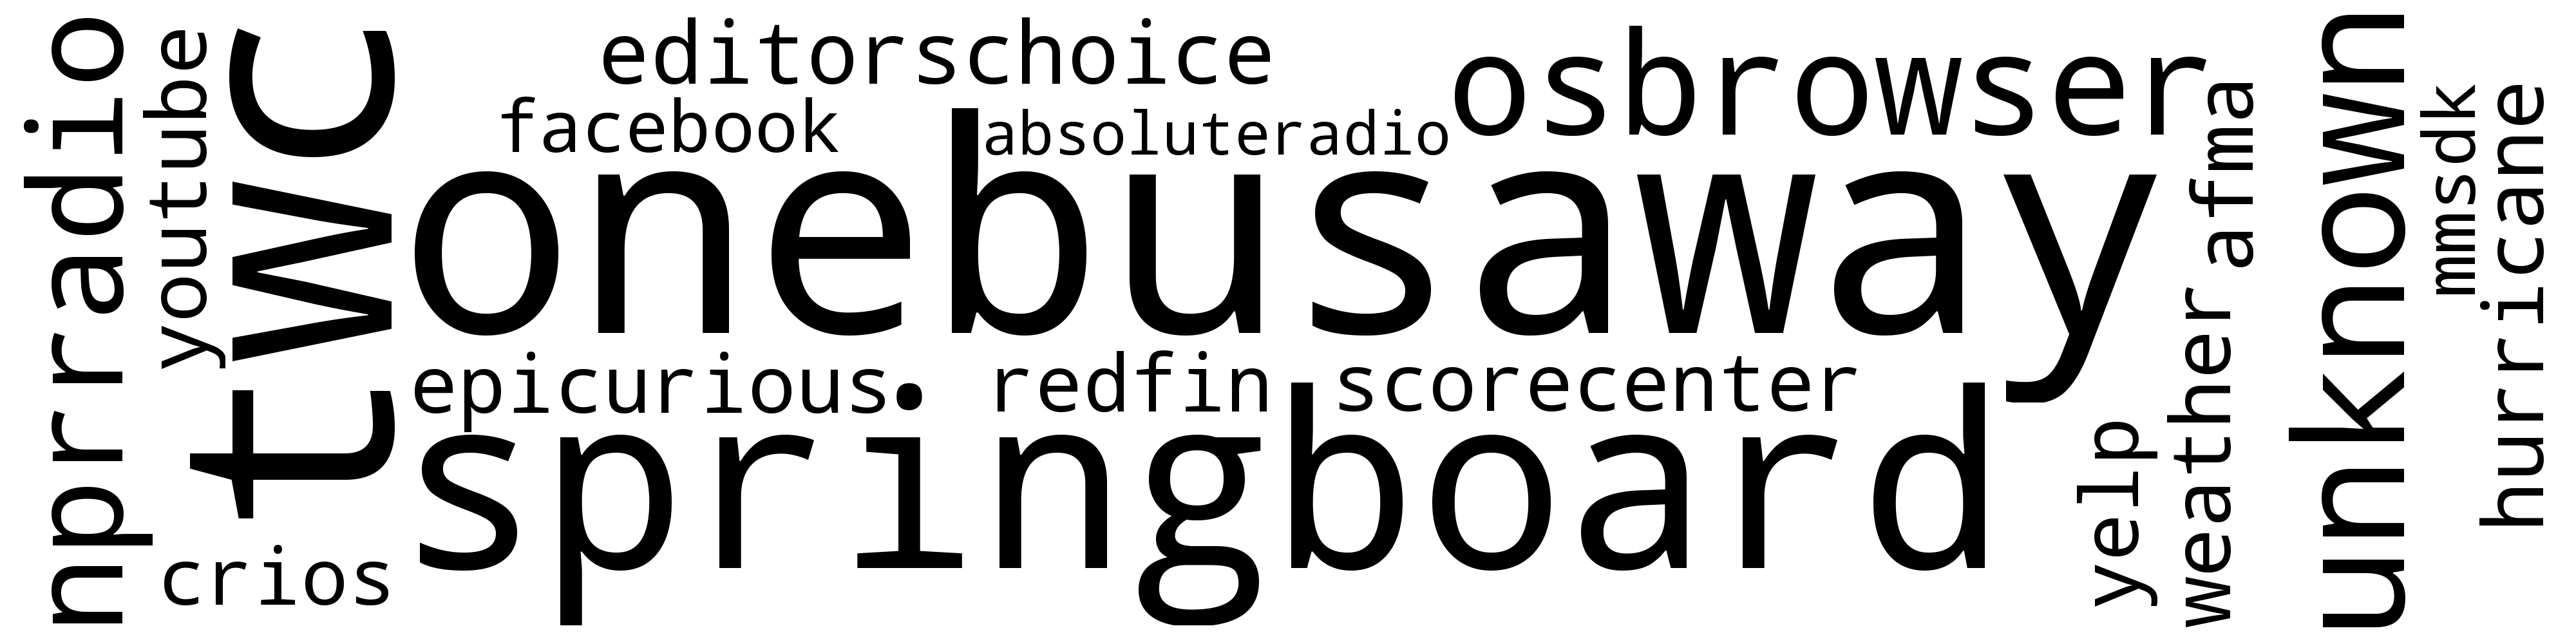
\includegraphics[width=\columnwidth]{figures/wordcloud_useragentsignature_location_image.png}
\caption{Applications that send the location information in the clear. \emph{The font size represent the number of flows that sent the location information in the clear.}}
\label{fig:location-wordcloud}
\end{figure}

In \fref{fig:location-wordcloud} we present a \emph{word cloud} of the applications that send the location information of the devices in the \mobWild dataset in the clear. 
We observe that a bus service application, \emph{One Bus Away}, the application that manages the iOS homescreen, \emph{springboard}, and  weather applications, \emph{twc}, \emph{weather}, and \emph{hurricane} were responsible for more 78\% of the flows that sent the location information in the clear. 
On further analysis, we observe that 4\% of the flows sent the location information to ads and analytics sites; more than 80\% of \emph{ad-flows} leaking location information did not include the an application signature in the user-agent field, the rest of the flows were from apps including, browsers, facebook, and angry birds.

Along with the location, we also observed that the device ID and IMEI number are leaked in the clear in the \mobWild dataset. 
Based on our classification methodology we observe that the IMEI number and device ID was leaked primarily through the Web-browser; we did not observe any application signature in non-browser flows in the \mobWild dataset that leaked the IMEI number or the device ID in the clear. 
As in the case of controlled experiments, ads and analytics sites were the most popular destination for the IMEI number leaks.
Among the 16 sites that sent the IMEI number in the clear, only 10 sites were ads and analytics sites; the rest of the sites included sites for games, news, and manufacturer updates.

%Similarly, from the device of one of the authors of the paper, we observed that the latest three versions YahooMail application, up to the time of the measurements, leaked the user's email address in the clear.




%\tbd{This should come before 
%We first identify A\&A flows using the publicly available database of~\cite{YoyoAds}; we augment this list of domains using recent research on mobile ads~\cite{hornyack:appfence, leontiadis:mobileads}.
%Based on this classification, we observe that the ads and analytics traffic was responsible for up to 6\% of the traffic by volume per device, an observation in line to the one made by Vallina-Rodriguez~\etal~\cite{vallina-rod:ads}}.

%\subsection{Ads and Analytics in the Wild}

We now focus our attention on the extent to which devices in the \mobWild dataset contact ads and analytics (A\&A) sites, an activity that is receiving considerable attention~\cite{roesner:webtrackers,leontiadis:mobileads,vallina-rod:ads}.
Using our classification based on the \httphost, we observe that the ads and analytics traffic was responsible for up to 6\% of the traffic by volume per device, an observation in line to the one made by Vallina-Rodriguez~\etal~\cite{vallina-rod:ads}.
Rather that focusing on the traffic volume we focus on the extent to which these sites are able to track the users in the dataset and the applications that facilitate this tracking. 

\begin{table}
\centering
\begin{small}
\begin{tabular}{|p{0.35\columnwidth}|p{0.1\columnwidth}|p{0.15\columnwidth}|p{0.1\columnwidth}|}
\hline
\multirow{2}{*}{\bf Tracker} & \multicolumn{3}{c|}{\bf Number of devices tracked}\tabularnewline
\cline{2-4}
                      &  {\bf Total} & {\bf iOS} & {\bf Android} \tabularnewline
\hline
doubleclick.net       & 26 {\em(all)} & 15 {\em(all)} & 11 {\em(all)} \tabularnewline
\hline
google-analytics.com  & 26 {\em(all)} & 15 {\em(all)}  & 11 {\em(all)} \tabularnewline
\hline
googlesyndication.com & 22 & 12 & 10 \tabularnewline
\hline
admob.com             & 21 & 11 & 10 \tabularnewline
\hline
scorecardresearch.com &  21 & 11 & 10 \tabularnewline
\hline
\end{tabular}
\end{small}
\caption{The top 5 ads and analytics sites that were contacted by the devices in our dataset.
\emph{The sites, doubleclick.net and google-analytics.com, were contacted by all the 26 devices in} \mobWild.}
\label{tab:top-trackers}
\end{table}

In \fref{tab:top-trackers} we present the number of A\&A sites ordered according to the number of devices that contacted them.
We observe that all the devices in the \mobWild dataset contacted doubleclick.com, an ad site, and google-analytics.com, a tracking site.
Furthermore, we observe that 66.12\% of the volume of ad traffic in the \mobWild dataset was from the browsers, 6.46\% of the traffic contained a blank user-agent field, and 4.8\% of the traffic contained a signature of \emph{Google-Analytics}\footnote{This signature was observed even in the flows for users that did not have the Google Analytics application installed on the device.}.
The rest of the traffic contained signatures of other applications such as Facebook, Pandora, and YouTube.
%\tbd{This must come before Furthermore, we observed that 7\% of the traffic contained the Google-Analytics in the signature field; this signature was observed even in the flows for users that did not have the Google Analytics application installed on the device. Mention that we will wrongly classify the flows from Google Analytics app as ads and analytics traffic} 




%%% Local Variables: 
%%% mode: latex
%%% TeX-master: "main"
%%% End: 

%       getjar.com     & - S & - S \tabularnewline
%       aarki.net      & - S & - - \tabularnewline
%       chartboost.com & - S & - S \tabularnewline
%       *pocketexchange&   S &   S \tabularnewline
%       *vserv.mobi    & - - & C   \tabularnewline
%       *groupon.com   &     &   S
%       *flurry.com    &     &   S
%       *bankofamerica &     &   S
%       *google.com    & - - & - S

\section{MISC}

% \begin{figure}
% \centering
% \includegraphics[width=\columnwidth]{plots/ads_wild_gatracking.pdf}
% \caption{Number of devices tracked by Google-Analytics. \emph{We observe that devices }}
% \label{fig:tracking-analytics}
% \end{figure}

% \begin{figure}
% \centering
% \includegraphics[width=\columnwidth]{plots/ads_wild_usertracking.pdf}
% \caption{Number of sites that track a user. \emph{We observe that devices }}
% \label{fig:tracking-analytics}
% \end{figure}

% \begin{figure}
% \centering
% \includegraphics[width=\columnwidth]{plots/ads_wild_sitescontacted.pdf}
% \caption{Number of visits to A\&A sites per device. \emph{The error bars indicate the 25$^{th}$ and 75$^{th}$ percentiles. Each visit is a potential tracking visit.}}
% \label{fig:tracking-analytics}
% \end{figure}

% \begin{table}    
%     \centering
%     \begin{small}
%     \begin{tabular}{|l|c|c|}
%        \hline
%        {\bf Host}&{\bf IMEI}&{\bf Device ID}\tabularnewline
%        \hline              
%        tapjoyads.com  & Y & - \tabularnewline
%        zynga.com      & Y & - \tabularnewline
%        iheart.com     & Y & Y \tabularnewline
%        google.com     & - & Y \tabularnewline
%        flurry.com     & - & Y \tabularnewline
%        \hline
%     \end{tabular}
%     \end{small}
%     \caption{Hosts to which the IMEI or Device ID was sent in the clear and over HTTPS. \emph{The value Y for a column implies that data was sent over HTTP and HTTPS. We order these hosts based on the number of flows that sent the IMEI number in the clear and over HTTPS.}}
%     \label{tab:pii-leakage-sites}
% \end{table}
